%==============================================================================    
\chapter{Silicon theory}
\label{sec:SiliconTheory}
%==============================================================================    
\section{Properties of semiconductor material}

\subsection{Band structure}
Due to periodic lattice of crystalline structure of semiconductor material, electrons within the solid have allowed energy bands. The energy of the electrons is confined to one of the energy bands. The bands may be separated by ranges of forbidden energies.

\begin{figure}[H]
  \centering
  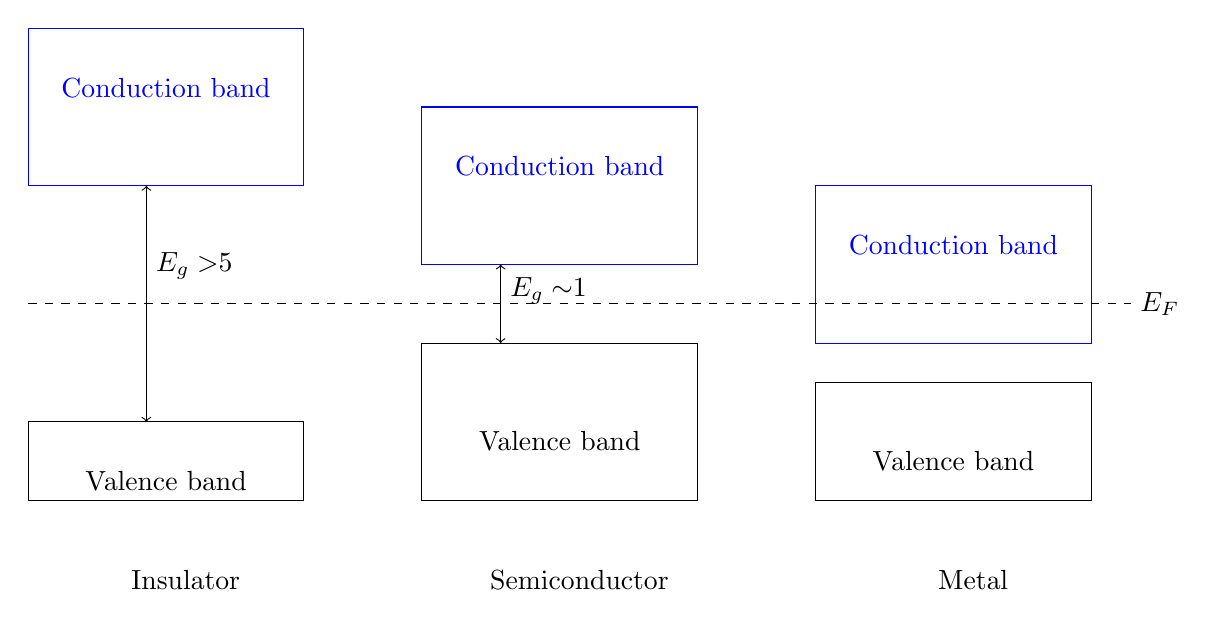
\begin{tikzpicture}
    \begin{scope} % Valence and conduction bands
      %  ----- insulator ----- %
        \draw (0, 1) rectangle node[below] {Valence band}  ++ (3.5, 1);
        \draw[blue] (0, 5) rectangle node[above] {Conduction band} ++ (3.5, 2);
        \node at (2, 0) {Insulator};

        % ----- Semiconductor ----- %
        \draw (5, 1) rectangle node[below] {Valence band}  ++ (3.5, 2);
        \draw[blue] (5, 4) rectangle node[above] {Conduction band} ++ (3.5, 2);
        \node at (7, 0) {Semiconductor};

        % ----- Metal ----- %
        \draw (10, 1) rectangle node[below] {Valence band}  ++ (3.5, 1.5);
        \draw[blue] (10, 3) rectangle node[above] {Conduction band} ++ (3.5, 2);
        \node at (12, 0) {Metal};
    \end{scope}


    \begin{scope} % Energy levels
        \draw[dashed] (0, 3.5) -- (14, 3.5) node[right] {$E_{F}$};
        \draw[arrows=<->](1.5, 2)--(1.5, 5) node [pos=0.66,right] {$E_{g}>$\SI{5}{\electronvolt}};
        \draw[arrows=<->](6, 3)--(6, 4) node [pos=0.66,right] {$E_{g}\sim$\SI{1}{\electronvolt}};
    \end{scope}

  \end{tikzpicture}
  \caption{}  \label{fig:energyBands}
\end{figure}


\section{Detector systems}

Figure~\ref{fig:basicDetectorFunction}, schematically summarises the sequence of basic detector functions.


\begin{figure}[H]
  \centering
  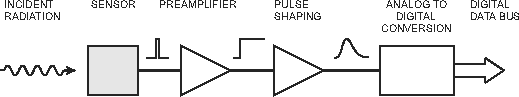
\includegraphics[width=\textwidth]{figures/basicDetectorFunction.png}
  \caption{The sequence of basic detector functions. From~\cite{Spieler2005}.}
  \label{fig:basicDetectorFunction}
\end{figure}


\subsection{Sensor} 
A silicon sensor, converts the energy deposited by a particle to an electric signal by producing electron-hole pairs. By applying an electric field to the sensor, the produced pairs are con
\subsection{Preamplifier}
\subsection{Pulse shaper}
\subsection{Digitiser}


\subsection{Charge transport in Silicon}
The potential $\varphi$ at each point is described by Poisson's equation~\ref{eq:poisson} \cite{Knoll2010}
\begin{equation}
\nabla^{2}  \varphi=-{\rho \over \epsilon}\; ,
\label{eq:poisson}
\end{equation}

where $\epsilon$ is the dielectric constant of the medium and $\rho$ the net charge density.
The electric field E due to the electric potential is obtained by Equation~\ref{eq:Efield}

\begin{equation}
E=-grad \varphi \; ,
\label{eq:Efield}
\end{equation}

In one dimension, Equation~\ref{eq:poisson} becomes
\begin{equation}
{{d^{2}  \varphi(z)} \over {dz^{2}}}=-{\rho(z) \over \epsilon}\; ,
\label{eq:poisson1D}
\end{equation}

To simplify, we assume an abrupt junction where the charge densities on the p and n sides are:
\begin{equation}
  \rho(z)= 
  \begin{cases} 
    eN_{D}, & \mbox{if } 0\leq z < z_{n}\\ 
    -eN_{A}, & \mbox{if } z_{p}\leq z < 0 
  \end{cases} 
  \; ,
\label{eq:chargeDensity}
\end{equation}

First, considering the n-side, the first and second integrations of the Poisson equation give,
\begin{equation}
    {{d\phi(z)} \over {dz}}=-{{eN_{d}} \over \epsilon} (z-z_{n}) 
    \; ,
    \label{eq:PoissonIntegration1}
  \end{equation}

\begin{equation}
  \phi(z)=-{{eN_{d}} \over \epsilon} {z^{2} \over 2}+{{eN_{d}zz_{n}}\over \epsilon}+Vj
  \; ,
  \label{eq:PoissonIntegration2}
\end{equation}

Where $V_j$ is the potential at the interface where the n- and the p-sides join. At the boundary of the depletion region $z=z_{n}$:

\begin{equation}
  \phi(z_{n})=V_{b}={{eN_{d}z_{n}^{2}} \over \epsilon}+V_j 
  \; ,
  \label{eq:BounderyPotential}
\end{equation}

In the p-region,
\begin{equation}
  V_j={{eN_ax_p^2} \over {2\epsilon}}
  \; ,
\end{equation}

And the total potential,
\begin{equation}
V_b={{e} \over {2 \epsilon}}(N_dx_n^2+N_ax_p^2)
  \; ,
\end{equation}

The overall charge neutrality is maintained,
\begin{equation}
N_d x_n=N_a x_p
  \; ,
\end{equation},

the reverse bias potential can be expressed as

\begin{equation}
V_b={e \over {2\epsilon}}\left(1+{N_a \over N_d}\right) N_a x_p^2={e \over {2\epsilon}}\left(1+{N_d \over N_a}\right) N_d x_n^2
  \; .
\end{equation}

The depletion widths on the n- and p-sides of the junction are

\begin{equation}
  \begin{multlined}
x_n=\sqrt{{2 \epsilon V_b} \over {eN_d(1+N_d/N_a)}} \\
x_p=\sqrt{{2 \epsilon V_b} \over {eN_a(1+N_a/N_d)}} 
\; ,
\end{multlined}
\end{equation}

The total depletion width is 

\begin{equation}
W=x_n+x_p=\sqrt{{2 \epsilon V_b \left(N_a+N_d\right)} \over {eN_aN_d} }
\; ,
\end{equation}

The junction potential and also for an asymmetrical junction with $N_d \ll N_a$ for which the junction potential is equal to the potential of the p-contact.

\begin{equation}
V_j=\left(N_d \over N_a\right) {V_b \over \left(  1+N_d/N_a \right)} \stackrel{N_d \ll N_a}{\approx} {N_d \over N_a}V_b
\; ,
\end{equation}


For a pixel detector with asymmetric junction with a highly doped surface $N_c$ concentration and a lightly doped bulk $N_b$ ($N_b \ll N_c$), the doping concentration is expressed in terms of resistivity 
\begin{equation}
\rho_b = {1 \over {e\mu_{b}N_{b}}}
\; ,
\end{equation}
where $\mu_b$ and $N_b$ are the mobility and the doping concentration of the bulk. The depletion width $W$ becomes,
\begin{equation}
W=\sqrt{2 \epsilon \mu_b \rho_bV_b}
\; ,
\label{eq:depletionWidth}
\end{equation}

In the absence of an externally applied voltage to a pn-junction, the thermal diffusion of the electrons and the holes from their original atoms results in a depletion width with a potential difference between the p- and n-sides called the built-in potential $V_{bi}$ which is about 0.5~V for detector diodes. \\
By taking into account the built-in reverse bias voltage, Equation~\ref{eq:depletionWidth} is written as,
\begin{equation}
W=\sqrt{2 \epsilon \mu_b \rho_b \left(V_b+V_{bi}\right)}=\sqrt{{2 \epsilon \left(V_b+V_{bi}\right)} \over {eN_b}}
\; ,
\label{eq:depletionWidth2}
\end{equation}

The electric field of Equation~\ref{eq:PoissonIntegration1}, by replacing the depletion width and $N_d$ by Equation~\ref{eq:depletionWidth2} can be expressed as
\begin{equation}
E(z)={{2\left(V_b+V_{bi}\right)} \over {W}} \left({z \over W}-1\right)
\; ,
\end{equation}

The depletion voltage ($W=d$) can be expressed as,
\begin{equation}
V_D={{eN_bd^2} \over {2 \epsilon}}-V_{bi}
\; ,
\label{eq:depletionVoltage}
\end{equation}
where $d$ is the detector thickness. \\

The electric field drops linearly from its maximum value at the junction to zero at the opposite contact. Increasing the bias voltage beyond the needed bias to completely deplete the detector adds a uniform field. By neglecting the built-in voltage (as the bias voltage is much higher than that), the electric field is written as,
\begin{equation}
E(z)={{V_B-V_D} \over d}+\left(1-{z \over d}\right)2{V_D \over d}
\; ,
\label{eq:Efield}
\end{equation}

The charge carriers, drift through the silicon detector with a velocity as defined by,

\begin{equation}
  \vec{v}_{drift}=\mu_c \cdot \vec{E}\; ,
\end{equation}

In one-dimension, and considering $\mu_c$ constant, the drift velocity is written as
\begin{equation}
v_{drift}={{dz} \over {dt}}=\mu_c \cdot E(z)
\; ,
\end{equation}

The time required for a charge originating at point $z_0$ to reach a point $z$ is
\begin{equation} 
  t(z)=\int_{z_0}^{z} {{ds} \over {\mu_c \cdot E(s)}}
  \; ,
  \label{eq:driftTimeIntegral}
\end{equation}

By integrating Equation~\ref{eq:driftTimeIntegral} and replacing the electric field by Equation~\ref{eq:Efield} one obtains:

\begin{equation} 
  t(z, z_0)={{d^2} \over {2 \mu_c V_D}} ln\left( {{d(V_B+V_D)-2V_Dz_0} \over {d(V_B+V_D)-2V_Dz}} \right)
  \; ,
  \label{eq:driftTimeIntegratedz0}
\end{equation}

In Equation~\ref{eq:driftTimeIntegratedz0}, by replacing $z_0=0$, we obtain:
\begin{equation} 
  t(z)={{d^2} \over {2 \mu_c V_D}} ln\left( {{V_B+V_D} \over {V_B+V_D-2V_Dz/d}} \right)
  \; ,
  \label{eq:driftTimeIntegrated}
\end{equation}

And the diffusion sigma is given by,

\begin{equation} 
  \sigma_{diffusion}\left(z\right)=\sqrt{2 D_{b} t_{c}}=\sqrt{{{kTd^2}\over{eV_D}}ln\left({{V_B+V_D}\over{V_B+V_D-2V_Dz/d}}\right)}
  \; ,
  \label{eq:driftTimeIntegrated}
\end{equation}

%% --------------------------------------------------- %%
% Carriers move in random direction due to the thermal energy. \\
% Material-dependent diffusion constant given by the Einstein equation:  

% \begin{equation}
%   D_{b}={{k_{B} \cdot T \cdot \mu_{c}} \over {e}}
% \end{equation}
% where \(k=8.617 3324\) is the Boltzman constant.

% \begin{equation}
%   \sigma_{diffusion}=\sqrt{2 \cdot D_{b} \cdot t_{c}}
% \end{equation}



